\documentclass[12pt]{report}
\usepackage[utf8]{inputenc}
\usepackage{graphicx}
\graphicspath{ {images/} }
\usepackage{biblatex}
\addbibresource{references.bib}
\pagenumbering{arabic}
\usepackage{amsmath}
\usepackage{pseudocode}
\linespread{2}
\usepackage{amsthm}
\usepackage{amssymb}
\newtheorem{theorem}{Theorem}[section]
\theoremstyle{named}
\newtheorem*{namedtheorem}{Theorem}

\title{
{Quantum Solution To Matrix Riccati Differential Equation: Preliminary Studies}\\
{\large Marist College}\\
\vspace{5mm}
{
\includegraphics[scale=0.1]{images/Marist_College_Seal_-_Vector.svg_.png}}
}
\author{Augusto Gonzalez-Bonorino}
\date{\today}

\begin{document}

\maketitle

\chapter*{Abstract}
Solving large linear systems is a task ubiquitous in science. At the time of writing the most efficient method is called the Conjugate Gradient method with complexity $O(N \cdot s \cdot k \cdot log(\frac{1}{\epsilon})$. Nevertheless, this approach soon hit a ceiling with Big Data and massive data sets. Quantum algorithms have been recently proposed to handle these high-dimensional data sets. In 2009, Harrow-Hassidim-Lloyd from MIT presented a quantum algorithm to approximate the function of the solution large linear systems with complexity $\frac{O(log(N) \cdot s^2 \csot k^2}{\epsilon}$, given the system meets certain conditions. Unfortunately, quantum hardware must be improved to reliably exploit the exponential advantage they claim. Hence, growing emphasis has been recently placed in hybrid architectures, composed of both a classical and a quantum component, better suited for small quantum computers. Here, we propose a mathematical proof and a hybrid algorithm to solve a high-dimensional Matrix Riccati equation using IBM's quantum lab and HHL solver package. 

\chapter*{Acknowledgements}
I want to thank Marist College School of Mathematics and Computer Science for offering one of the first courses in Quantum Computing, and Dr. Casimer DeCusatis for teaching it, in partnership with IBM last semester. The ideas presented in this thesis would have never become a reality if it wasn't for the early introduction to quantum computing the College provided. Also, I would like to thank Dr. Malick Ndiaye for his guidance on the mathematical proofs presented in this paper, his help made this project feasible in a semester. Lastly, I want to thank my parents for their continuous love and support, specially throughout these past few years at Marist College. They deserve as much credit for my achievements as I do.

\tableofcontents

\chapter{Introduction} Count Jacopo Francesco Riccati (1676-1754) is the mathematician, along with Giovanni Poleni and Bernardino Zendrini, credited with developing the now fundamental family of Riccati Differential Equations \cite{jungers_historical_2019}. Interested in problems related to plane curves determined by curvature properties, Riccati showed that the solution curve arises from a second order differential equation after applying a suitable change of variables \cite{riccati_soluzione_nodate}. This discovery led him to four particular solutions, which arguably marked the beginning of the famous Riccati equations. Eager to find more solutions to his equation, Riccati decides to reach out to his mentor, Poleni, asking to share his work with Nicolas I Bernoulli \cite{riccati_letter_1718} and Christian Goldbach. Goldbach’s and Bernoulli's family expertise played a crucial role in further developing methods to solve this new interesting equation that Francesco Riccati has proposed. Work that culminated in a paper published in 1724 titled “Animadversiones in aequationes differentiales secundi gradus”, by Jacopo F. Riccati \cite{riccati_animadversiones_1724}.


In general, a Ricatti equation is any differential equation involving a constant, a linear and a quadratic term. We can “factor” this general definition into two common sub-categories: Scalar and Matrix form. A scalar Riccati differential equation is of the form:
\begin{equation}
    y'(t) = a(t)\cdot y(t)^2 + b(t)\cdot y(t) + c(t)
\end{equation}
where y(t) is the dependent variable, t stands for time and a,b and c are coefficients. Alternatively, we can extrapolate the scalar form into a Matrix equation of the following form:
\begin{equation}
    Y'(t) = Y(t)\cdot A(t) + D(t) \cdot Y(t) + Y(t) \cdot B(t) \cdot Y(t) + C(t)
\end{equation}
defined on the vector space of real m x n matrices, and where A,B,C and D are real matrix functions. Two recent findings about the nature of these equations will prove useful in our case study. First, it can be shown that any nonlinear Riccati scalar differential equation can always be converted to a second order linear ordinary differential equation (ODE). Furthermore, it follows that any nonlinear Matrix Riccati equation can be converted to a system of second order linear ODEs. We will leverage the latter in our case study to derive a Hermitian matrix suitable to serve as input to the HHL quantum algorithm for linear systems (details provided in following sections).

Matrix Riccati Differential Equations have a vast array of applications throughout many different disciplines ranging from physics and electrical engineering, to game theory \cite{toivonen_chapter_2}. Among the most useful applications of this particular form of Riccati equations we find optimal control, random processes, stochastic realization theory and quantum mechanics. 

Interestingly, Riccati equations possess special characteristics that have proven useful in unifying linear quantum mechanics and related fields of physics, such as thermodynamics and cosmology \cite{schuch_nonlinear_2014}. This suggests that solving Matrix Riccati equations is a suitable task for a quantum computer.

Before considering quantum solutions though, a word of caution must be made. To date there is no general recipe to find solutions to Riccati equations. Nevertheless, if a particular solution is obtained then it is always possible to derive the general solution by applying a special change of variables that yields a Bernoulli equation \cite{dawkins_bernoulli_2018}. Consider the following to illustrate this technique:

Consider the general Riccati equation
\begin{equation}
    y' = a(t)\cdot y^2 + b(t)\cdot y + c(t)
\end{equation}
where a(t), b(t) and c(t) are continuous functions of t.
\\
Now, suppose we have a particular solution $y_1$ to this general equation. Then, we can make the following change of variables
\begin{equation}
    y = y_1 + u
\end{equation}
and so we can re-write the general equation as
\begin{equation}
    \begin{split}
        (y_1 + u)' & = a(t)\cdot (y_1 + u)^2 + b(t)\cdot (y_1 + u) + c(x)\\\\
        y_1' + u' & = a(t)\cdot (y_1^2 + 2\cdot y_1 \cdot u + u^2) + b(t)\cdot y_1 + b(x)\cdot u + c(t)\\\\
        y_1' + u' & = a(t)\cdot y_1^2 + a(t) \cdot 2\cdot y_1 \cdot u + a(t)\cdot u^2 + b(t)\cdot y_1 + b(t)\cdot u + c(t)
    \end{split}
\end{equation}
It follows that, since $y_1$ is a particular solution to the Riccati equation we can cancel out $y_1'$, $a(t)\cdot y_1^2$, $b(t)\cdot y_1$ and $c(t)$. Hence, we obtain
\begin{equation}
    \begin{split}
        u' & = a(t)\cdot u^2 + u\cdot [2\cdot a(t)\cdot y_1 + b(t)]\\
        u' - u\cdot [2\cdot a(t)\cdot y_1 + b(t)] & = a(t)\cdot u^2\\
        \frac{u'}{u^2} + [-2\cdot a(t)\cdot y_1 - b(t)]\cdot \frac{1}{u^2} &= a(t)
    \end{split}
\end{equation}
Note that $u'$ is a Bernoulli equation and thus we can apply well-established methods to find the general solution. First, we make the substitution $z = u^{1 - m}$, where $m = 2$ in this case, to transform the Bernoulli into the following \underline{linear differential equation}:
\begin{equation}
    -z' + [-2\cdot a(t)\cdot y_1 - b(t)]\cdot z = a(t)
\end{equation}
These methods and ideas can be expanded to Matrix form, by translating our simple calculus to Matrix Calculus.



\chapter{Quantum Computing in a Nutshell}
\section{Historical Background}
I believe that reviewing the challenges and actors that played a key role in the development of Quantum Computing is necessary for a comprehensive understanding of this nascent technology's true potential. In the following paragraphs I will attempt to illustrate the birth of Quantum Computing, in a nutshell. 

The first fundamental breakthrough in the development of Quantum Mechanics came from the related area of Chemistry during the early 19th century. John Dalton's atomic theory, which states that elements are composed by identical and indivisible particles we know call atoms \cite{daltons_2014}. Dalton's discovery opened the door for curious physicists of that era to ponder about the nature of these atoms and their role in our universe. One hundred years passed until the nascent theory of quantum mechanics experienced another breakthrough of such magnitude. In the early 1900s, German theoretical physicist Max Planck observed an extraneous pattern in the information outputted by his measurement tools. From this subtle observation Planck developed his famous Planck's law, which postulates that the electromagnetic energy is emitted not continuously, unlike classical physics which assumes this to be true, but by discrete portions or quants \cite{khairoutdinov_plancks_2012}.

Danish physicist Nielhs Bohr used Planck's work to gain a deeper understanding of atoms and their behavior. Along with his protégés, such as Enrico Fermi and Werner Heisenberg, Bohr lead a revolutionary movement within the world of Physics powered by mind-blowing scientific discoveries \cite{loeffler_niels_2018}. The concepts of superposition, entanglement and the wave-particle duality model were developed. Quantum Mechanics was born. Although novel, most physicists of the time considered their ideas ridiculous or incomprehensible. Among the most famous critics of Bohr's work we find Albert Einstein, who failed to make sense of the probabilistic universe quantum mechanics was proposing. Multiple spirited discussions were exchanged between them until Einstein, Podolsky and Rosen proved their famous EPR paradox \cite{epr_paradox}, which supported the entanglement theory that Bohr's was proposing.

\section{Feynman's vision and the Quantum Turing Machine (QTM)}

By the 1950s Quantum Physics was a well-established sub-discipline of Physics that focuses in understanding the characteristics and behavior of atoms. Efforts proved very successful. Among the plethora of advancements credited to quantum mechanics there is the manipulation of chemical reactions, ideas that fueled the development of the atomic bomb during the 1940s. But, the Manhattan Project left us with something else besides an atomic bomb and a deeper understanding of quantum objects: Richard Feynman. With less than 30 years of age, Dr. Feynman was in charge of running the computing unit responsible for making the calculations behind the first atomic bombs \cite{selwood_richard_2018}. After receiving the Nobel Prize in Physics in 1965, alongside Sin-Itiro Tomonaga and Julian Schwinger, "for their fundamental work in quantum electrodynamics, with deep-ploughing consequences for the physics of elementary particles." \cite{nobel_physics} Dr. Feynman embarked on a new challenge: Simulating quantum phenomena. 

Curious about the limitations of classical computers governed by the laws of Physics and the possibility of simulating Nature, Richard Feynman proposed in 1980 a radical computer architecture based on the laws of quantum mechanics \cite{feynman_simulating_1981}. The problem was that the world we inhabit is inherent probabilistic, yet computers were deterministic by definition. Thus, we are left with two logical options: Design a probabilistic computer or figure out a way to design a classical universal automaton capable of this kind of simulations. 

This novel architecture, now called Quantum Computing, exploits ideas of quantum physics like superposition, linear association amongst qubits' states, and entanglement, a peculiar correlation between two particles (i.e. qubits) regardless of how far apart they are from each other, to process high dimensional computations more efficiently. For instance, consider the task of folding a protein. A supercomputer would try to check every single combination the protein could adopt, an approach that grows exponentially in complexity as the size of the protein increases. In contrast, a Quantum Algorithm proceeds by creating multidimensional spaces where the patterns linking individual data points emerge \cite{ibm_quantum}. Nevertheless, current quantum computers, called Noisy-Intermediate-Scale-Quantum (NISQ) computers, are very sensitive to changes in the environment, like heat fluctuations. Therefore, we are not able to retrieve a desired result with certainty. Understanding how to reduce the uncertainty, or interference, of quantum algorithms is being actively studied by the field of Quantum Error Correction \cite{somoroff_quantum_2018}.

Recently, there has been a growing focus on hybrid architectures. For instance, in March of 2022 researchers from Google Quantum AI proposed a framework to combine quantum algorithms with classical monte carlo simulation to study chemistry \cite{huggins_hybrid_2022}. These are algorithms composed of both a classical and a quantum component. By taking advantage of quantum hardware, we can process computationally expensive subroutines of a classical algorithm with a smaller, noisy, quantum algorithm more efficiently. Hence, the overall performance of the architecture increases. In this thesis I propose a novel hybrid architecture for approximating solutions to systems of linear equations, that combines an existing quantum algorithm with classical procedures, and apply it to solving a Matrix Riccati equation.

\chapter{Theory}

\section{Quantum Linear System Problem (QLSP)}

The "Classical" Linear System Problem (LSP) states the following:
\\
Given an $N \times N$ matrix A, an $N-$dimensional vector $\Vec{b}$, and the equation
    \begin{equation*}
        A \Vec{x} = \Vec{b}
    \end{equation*}
solve for $\Vec{x} = (x_1, x_2,...,x_N)^T$. To date, the best algorithm for this task is called the Conjugate Transpose method first introduced by Hestenes and Stiefel in 1952 \cite{hestenes_methods_1952}. It has an asymptotic complexity of $O(N\cdot \sqrt{k})$, and thus complexity grows polynomially as the number of inputs increases. 

Analogously, the Quantum Linear System Problem (QLSP) states that given a Hermitian $N \times N$ matrix A, a unit vector $\Vec{b}$, and the equation
    \begin{equation*}
        A \Vec{x} = \Vec{b}
    \end{equation*}
prepare a quantum state that approximates
\begin{equation*}
    | x \rangle = \frac{\sum_{i=1}^N x_i | i \rangle}{\sqrt{(\sum_{i=1}^N | x_i |^2)}}
\end{equation*}
where $\Vec{x} = (x_1, x_2,...,x_N)^T$. Specifically, for a given precision $\epsilon > 0$, the approximate (mixed or pure) quantum state $\rho_x$ satisfies
\begin{equation*}
    \frac{1}{2}Tr|\rho_x - |x\rangle \langle x| | \leq \epsilon
\end{equation*}

\section{Quantum Algorithms for Solving Linear Systems}

A particular family of quantum algorithms leverage the powerful properties of subatomic particles, particularly superposition and entanglement, to approximate solutions to linear systems of equations. Arising from the wave-like behavior of particles, superposition refers to the ability of quantum state as a linear combination of other distinct quantum states. By distributing information stored among many qubits, each of which adopts many different states, superposition allows us to encode inputs with exponentially less resources, one of the most promising characteristics of quantum algorithms. In addition, when two particles get really close to each other their quantum states become interdependent; they become entangled. This characteristic allows quantum computers to massively distribute calculations among several entangled qubits. 

\subsection{HHL algorithm}

The Harrow-Hassidim-Lloyd (HHL) quantum algorithm, given a Hermitian matrix \textbf{A}, will compute the vector of unknowns $|x\rangle$ in the form $|x \rangle = \sum_{j=1}^N \beta_j \cdot \frac{1}{\lambda_j} |\textbf{u}_j \rangle$ where $\{ |\textbf{u}_j \rangle \}$ denotes the eigenvectors of A and $\{\lambda_j\}$ its eigenvalues. By encoding the amplitudes of the input information HHL only need polynomial logarithm of qubits with respect to the input size \cite{duan_survey_2020}. Then, HHL performs three important operations:
\begin{enumerate}
    \item Quantum Phase Estimation (QPE)
    \item Invert the eigenvalues
    \item Measurement
\end{enumerate}
QPE consists in estimating the phase of an eigenvalue of the unitary operator $U$ that we create by using the properties of Hermitian matrices. In Quantum Linear Solvers this phase is critical to efficiently compute, often by spectral decomposition, the input matrix's inverse and invert the eigenvalues in the eigenbasis of the given matrix during the second step. Finally, the algorithm measures the auxiliary qubit in the computational basis and if the outcome is 1, then the state of that qubit contains the solution. 

\begin{figure}[h!]
    \centering
    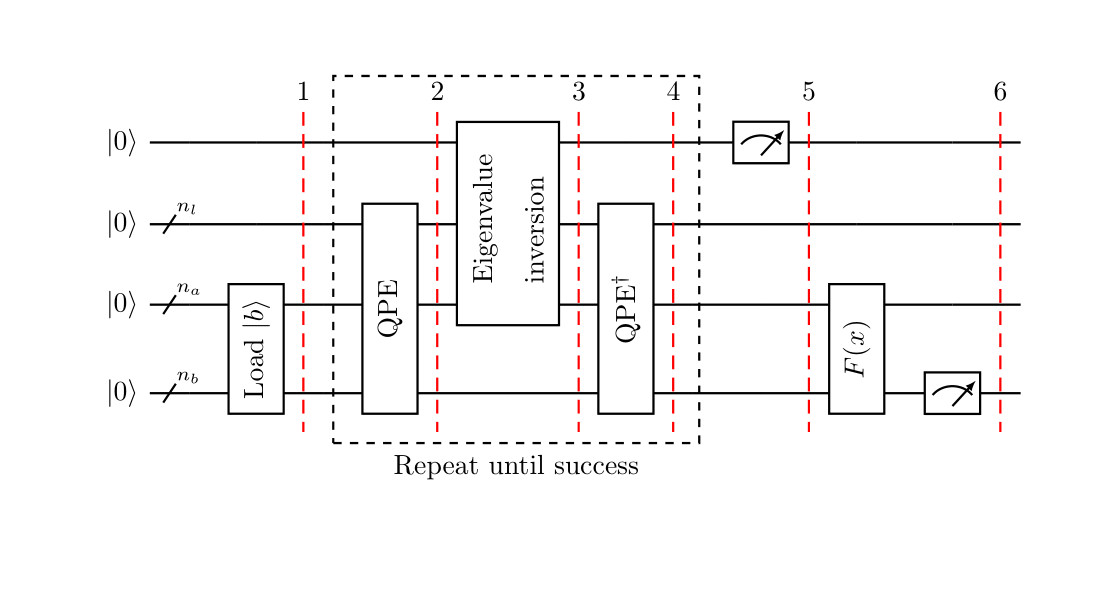
\includegraphics[scale=0.35]{images/hhlcircuit.png}
    \source{Source: \url{qiskit.org/textbook/ch-applications/hhl_tutorial.html}}
    \caption{HHL algorithm Circuit}
    \label{fig:my_label}
\end{figure}

The above graph depicts the circuit for HHL algorithm. After encoding the solution vector $|b \rangle$ as a linear combination of the input matrix A's eigenvectors, the algorithm undergoes an iterative process of inverting A's eigenvalues, by applying Quantum Phase Estimation with $U = e^{iAt}$, as well as computing A's inverse until the measurement (depicted in between lines 4 and 5) yields 1. Lastly, it returns the estimate $|\Tilde{x}\rangle \approx \sum_{j=1}^n \langle u_j|b \rangle / \lambda_j|u_j\rangle$ exponentially faster than the current best classical algorithm of conjugate gradient.

\section{A Hybrid Architecture to Solve the Riccati Equation}

The Matrix Riccati differential equation plays a key role in many applied fields including Control theory, theories of stabilization, transport theory, differential games and stochastic control.

I propose a hybrid algorithm to solve the Matrix Riccati differential equation given an initial condition. First, I show that some  Matrix Riccati equation can be turned to a linear system, given certain conditions are met, in which the matrix associated is Hermitian. Second, the mathematical findings are encoded in the classical component of the proposed algorithm. Third, I feed the Hermitian matrix output by step 1 to HHL on IBM's 4-qubit quantum computer, via IBM's quantum lab, and obtain the solution.

\subsection{Re-writing the Matrix Riccati equation}

Let R denote the following Matrix Riccati equation
\begin{equation}
\tag{R}
    Y' = Y\cdot A(t) \cdot Y + C(t)\cdot Y + Y\cdot B(t) + D(t)
\end{equation}
where $Y \in \mathbb{R}^{ n \times m}$, $D(t) \in \mathbb{R}^{ n \times m}$, $C(t) \in \mathbb{R}^{ n \times n}$, $B(t) \in \mathbb{R}^{m \times m}$ and $A(t) \in \mathbb{R}^{ m \times n}$.
The goal is, given an initial condition $Y(0)$, to obtain solutions $Y(t)$ for $t > 0$.

\begin{theorem}
Assuming $m = n$, if $B(t) = 0$ and if $A(t)$ is invertible, then R can be converted to the following second order matrix differential equation:
\begin{equation*}
    u'' - (ACA^{-1} + A'A^{-1})\cdot u' + AD \cdot u = 0
\end{equation*}

by using the change of variables $Y = - A^{-1} \cdot u' \cdot u^{-1}$, where $u$ is invertible. 
\end{theorem}

For conciseness, I will highlight the main steps of our proof, please refer to the Appendix for the full proof. 

\begin{theorem}
If $ACA^{-1} + A'A^{-1} = S$ where $S$ is a matrix with constant entries and diagonalizable, and $A \cdot D = -I$, then (R2) can be converted into the following equation:
    \begin{equation}
        \tag{R3}
        v'' - D_1 \cdot v' - v = 0
    \end{equation}
where $D_1$ is a diagonal matrix.
\end{theorem}


Please refer to the Appendix for the full proof. From (R3) we obtain the following linear system
\begin{equation}
    e^{-tM_{ii}} \cdot x_{ii} = w_{ii}
\end{equation}
where $M_{ii} = \big(\begin{smallmatrix}
      0 & 1\\
      1 & -\alpha_i
    \end{smallmatrix}\big)$, $\alpha_i$ denotes the entries in the diagonal of the matrix $D_1$, $w_{ii} = [v_{ii}(0), v'_{ii}(0)]^T$, where $v_{ij}$ are the entries of $v$ so $v = (v_{ij})$ and $1 \leq i,j \leq n$. 

Solving $e^{-tM_{ii}} \cdot x_{ii} = w_{ii}$ is equivalent of solving the system. 
\begin{equation*}
    H \cdot
    \begin{pmatrix}
        x_{11} \\
        x_{22} \\
        \vdots \\
        x_{nn}
    \end{pmatrix}
    = \Vec{w}
\end{equation*}
where 
\begin{equation*}
    H = \begin{pmatrix}
        e^{-tM_{11}} & 0 & 0 & ... & 0 \\
        0 & e^{-tM_{22}} & 0 & ... & 0 \\
        0 & 0 & e^{-tM_{33}} & ... & 0 \\
        0 & 0 & 0 & ... & e^{-tM_{nn}}
    \end{pmatrix}
    \text{and} \hspace{0.8mm} \Vec{w} = \begin{pmatrix}
        w_{11} \\
        w_{22} \\
        \vdots \\
        w_{nn}
    \end{pmatrix}
\end{equation*}

Note that $H$ is sparse and Hermitian for any $1 \leq i \leq n$. Thus, after normalizing the vector $\Vec{w}$, we can leverage the HHL quantum algorithm to gain an exponential advantage over current classical algorithms.


\chapter{A particular case of Matrix Riccati}

In the particular case where $m=n=1$, we get the following Riccati equation:
\begin{equation}
    \frac{dy}{dt} = A(t)y^2 + B(t)y + C(t)
\end{equation}
where $A(t), B(t), C(t)$ are real-valued functions of $t$. Given an initial condition $y(0)$, we want to compute $y(t)$.

First, we convert the Riccati equation to a second order differential equations by applying the change of variables $y = - \frac{v'}{A\cdot v}$, such that we obtain the following equation:
\begin{equation*}
    v'' + v' \cdot (B - \frac{A'}{A}) + A\cdot C\cdot v = 0
\end{equation*}
Next, let $\alpha = B - \frac{A'}{A}$ and assume $A\cdot C = -1$, which must hold for the resulting matrix to be Hermitian. From this, we obtain a system with vector of unknowns $\Vec{u} = [v, z]^T$ and a matrix $M = 
    \big(\begin{smallmatrix}
      0 & 1\\
      1 & -\alpha
    \end{smallmatrix}\big)$. Therefore, we obtain the following equation $u' = M\cdot u$. We proceed by computing the characteristic polynomial to obtain the following eigenvalues:
\begin{equation*}
    \lambda_i = \frac{-\alpha \mp \sqrt{\alpha^2 + 4}}{2}, i \in \{1,2\}
\end{equation*}
and thus the corresponding eigenvectors are:
\begin{equation*}
    V_1 = [1, \lambda_1]^T; V_2 = [1, \lambda_2]^T
\end{equation*}
Finally, we construct a Passage matrix $P = \big(\begin{smallmatrix}
      1 & 1\\
      \lambda_1 & \lambda_2
    \end{smallmatrix}\big)$, such that we can rewrite our matrix $M$ as $H = P \cdot D \cdot P^{-1}$ where $D = \big(\begin{smallmatrix}
      \lambda_1 & 0\\
      0 & \lambda__2
    \end{smallmatrix}\big)$ is a diagonal matrix.
    
It follows that to solve this system we must compute $\Vec{x} = e^{tH} \cdot x_0$, where $x_0 = [u(0), z(0)]^T$. Thus, we must rewrite the problem as $e^{-tH}\cdot \Vec{x} = x_0$, where $e^{-tH} = P \cdot e^{-tD} \cdot P^{-1}$. Since we now know $e^{-tH}$ is Hermitian, we conclude by normalizing $x_0$ such that $u(0)^2 + z(0)^2 = 1$.

\subsection{Quantum Riccati Solver (QRS)}

\begin{pseudocode}[shadowbox]{QRS}{A, A', B, initCondition, T}
    \IF A \cdot C \neq -1 \AND (B + \frac{A}{A'})' \neq 0
    \THEN $\text{Display error message. Halt program.}$\\
    $\alpha$ \GETS B + \frac{A}{A'}\\
    $\lambda_1$ \GETS $(\alpha + \sqrt{\alpha^2 + 4}) / 2 $\\
    $\lambda_2$ \GETS $\alpha - \sqrt{\alpha^2 + 4}) / 2  $\\
    $\text{Compute components of new matrix \textbf{M}}$\\
    $\text{Compute vector \textbf{x} of unknowns using initCondition}$\\
    $\text{Feed \textbf{M} and \textbf{x} to HHL}$\\
    $\text{Extract the right vector components from statevector \Psi}$\\
    $y_t$ \GETS -( $z(T) / ( A(\text{T}) \cdot u(T) ) $)\\
    \OUTPUT{$y_t$}
\end{pseudocode}

\textbf{Step 0 - Prepare inputs to feed QRS}
\begin{itemize}
    \item[-] The Quantum Riccati Solver (QRS) takes as input the values for the coefficients of the equation, the initial condition $Y(T)$ and the time $T$. 
\end{itemize}


\textbf{Step 1 - Check conditions:}
\begin{itemize}
    \item[-] QRS checks the required conditions are met. If not, the program displays the error and halts. To check that $\alpha$ is indeed a constant the algorithm check it's derivative equals zero and registers the variable as a Sympy constant Quantity \cite{sympy_2022}                                                                                                   
\end{itemize}

\textbf{Step 2 - Compute Eigenvalues:}
\begin{itemize}
    \item[-] QRS computes the eigenvalues $\lambda_i, i \in \{1,2\}$ of the system of equations we derived in the previous section.
\end{itemize}

\textbf{Step 3 - Compute Components of Hermitian matrix:}
\begin{itemize}
    \item[-] The eigenvalues are then utilized to compute the values of each component in our new matrix \textbf{M}. 
\end{itemize}

\textbf{Step 4 - Find Particular Solution}
\begin{itemize}
    \item[-] Solve for $\textbf{M}\cdot \textbf{x} = b$ to compute the normalized vector of unknowns $\textbf{x}$ for the specified initial condition $Y(0)$ by calculating the values of its components $x_0 = \frac{1}{\sqrt{1 + A(0)^2 + Y(0)^2}}$ and $x_1 = - \frac{A(0)\cdot Y(0)}{\sqrt{1 + A(0)^2 + Y(0)^2}}$
\end{itemize}

\textbf{Step 5 - HHL}
\begin{itemize}
    \item[-] Feed \textbf{M} and \textbf{x} to HHL to find the solution to the given system. This is achieved by extracting the statevector $\Psi$, containing the quantum state of each qubit, from the circuit generated by the quantum computer.
\end{itemize}

\textbf{Step 6 - Return estimate of y(t)}
\begin{itemize}
    \item[-] Finally, QRS extracts the states of the qubits containing our answers and computes a numeric approximation of the solution by solving for $y_t = -(z(T) / ( A(\text{T}) \cdot u(T) ) $).
\end{itemize}

\chapter{Results}
To test the algorithm's performance I ran it with the following example:

Consider the following Riccati equation with initial condition $y(0) = 1$
\begin{equation*}
    \frac{dy}{dt} = (2 - sin(t)) \cdot y^2 + \frac{2 - sin(t) + cos(t)}{2 - sin(t)} \cdot y - \frac{1}{2 - sin(t)}
\end{equation*}

The following four figures visualize the results of both the classical solver (\textit{y(t)}) and QRS (\textit{z(t)}) over a time period \textit{t} with the classical yt-graph from Differential Equations.

Figure 5.1 depicts the solutions of a classical solver and Figure 5.2 the solutions of QRS for a time step of 0.001. Note that the equation has a singularity, a point in which the solution splits to $\infty$ and $-\infty$, at $t \approx 0.40$ which describes the end of our particular solution. 

\begin{figure}[b]
    \centering
    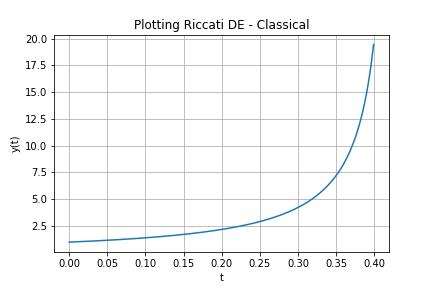
\includegraphics[scale=0.75]{images/Classical_R2.jpg}
    \caption{Classical solver qualitative analysis}
    \label{fig:my_label}
\end{figure}
\begin{figure}[b]
    \centering
    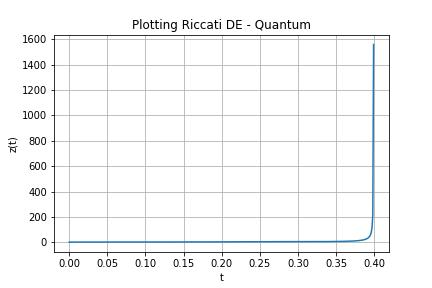
\includegraphics[scale=0.75]{images/Quantum_R2.jpg}
    \caption{Hybrid-Quantum solver qualitative analysis}
    \label{fig:my_label}
\end{figure}

Recall the Uniqueness and Existence theorem states that there is a unique solution for a given initial value problem within a local neighbourhood, defined by $\epsilon > 0$. Zooming into a local neighbourhood at (0.3, 0.375), Figure 5.3 and 5.4 show that QRS provides really good approximations over the specified region with a time step of 0.001.
\begin{figure}[b]
    \centering
    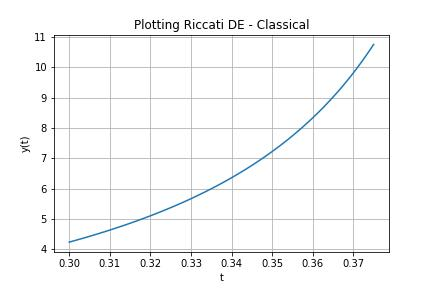
\includegraphics[scale=0.75]{images/Classical_R2_Zoom.jpg}
    \caption{Classical solution in local neighbourhood}
    \label{fig:my_label}
\end{figure}
\begin{figure}[b]
    \centering
    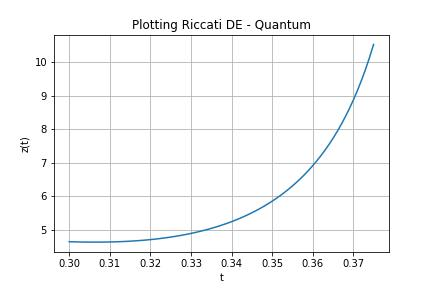
\includegraphics[scale=0.75]{images/Quantum_R2_Zoom.jpg}
    \caption{QRS solution in local neighbourhood}
    \label{fig:my_label}
\end{figure}

I believe the slight variations are mainly due to quantum noise and the singularities inherent to the equations chosen for evaluation. There has been some work on how to address singularities which seem to be common in Riccati equations, Davey \cite{DAVEY1979137} suggests that these could be removed by considering the differential equations for the numerators and the denominators separately of the elements of the Matrix Riccati and its inverse. My thought is that, while attempting to compute numbers growing to $\infty$ the quantum hardware heats up faster; I believe this alteration of the environment may affect the state of the qubits and thus the calculations. Therefore, QRS has a lot of room for improvement by applying error correction techniques and other quantum optimization methods. Further improvements will be discussed in the following section.

\chapter*{Conclusion}
In this project, some cases of the matrix Riccati equations have been considered. Specifically, the case where $B = 0$, $A \cdot D = -I$ and $A \cdot C \cdot A^{-1} + A' \cdot A^{-1} = S$ where $S$ is a matrix with constant entries and diagonalizable. We have presented a mathematical proof to show that solving large Matrix Riccati equations is indeed a suitable task for quantum computers. Moreover, the insights obtained from our mathematical analysis were encoded into the classical component of a hybrid architecture that, when coupled with HHL algorithm, shows promising results for solving such large linear systems. 

For further research, one can explore the cases where $S$ is not diagonalizable, $B \neq 0$ or the matrix $A$ is not invertible. Moreover, the quantum component of QRS can be improved in many dimensions. We intend to test modern hybrid architectures, optimize the program to run more efficiently on quantum hardware and explore the behavior of QRS when certain conditions are relaxed to generalize the model.

\printbibliography

\chapter*{Appendix}

Let R denote the following Matrix Riccati equation
\begin{equation}
\tag{R}
    Y' = Y\cdot A(t) \cdot Y + C(t)\cdot Y + Y\cdot B(t) + D(t)
\end{equation}
where $Y \in \mathbb{R}^{ n \times m}$, $D(t) \in \mathbb{R}^{ n \times m}$, $C(t) \in \mathbb{R}^{ n \times n}$, $B(t) \in \mathbb{R}^{m \times m}$ and $A(t) \in \mathbb{R}^{ m \times n}$.

\begin{namedtheorem}[Theorem 3.3.1]
Assume $m=n$. If $B(t) = 0$ and if $A(t)$ is invertible, then (R) can be converted to the following second order matrix differential equation:
\begin{equation}
\tag{E1}
    u'' - (ACA^{-1} + A'A^{-1})\cdot u' + AD \cdot u = 0
\end{equation}
by using the change of variables $Y = - A^{-1} \cdot u' \cdot u^{-1}$, where $u$ is invertible.
\end{namedtheorem}

\begin{proof}
\begin{equation*}
    Y' = -(A^{-1})' \cdot u' \cdot u^{-1} - A^{-1} \cdot u'' \cdot u^{-1} - A^{-1} \cdot u' \cdot (u^{-1})'
\end{equation*}
Recall $(A^{-1})' = - A^{-1} \cdot A' \cdot A^{-1}$. Then, 
\begin{equation*}
    \begin{split}
        Y' &= A^{-1} \cdot A' \cdot A^{-1} \cdot u' \cdot u^{-1} - A^{-1} \cdot u'' \cdot u^{-1} + A^{-1} \cdot u' \cdot u^{-1} \cdot u' \cdot u^{-1}\\
        &= A^{-1} \cdot u' \cdot u^{-1} \cdot A \cdot A^{-1} \cdot u' \cdot u^{-1} + A^{-1} \cdot u' \cdot u^{-1} \cdot B - C \cdot A^{-1} \cdot u' \cdot u^{-1} + D  
    \end{split}
\end{equation*}
It follows that, since $B(t) = 0$
\begin{equation*}
    \begin{split}
        Y' &= A^{-1} \cdot u' \cdot u^{-1} \cdot A \cdot A^{-1} \cdot u' \cdot u^{-1} - C \cdot A^{-1} \cdot u' \cdot u^{-1} + D
    \end{split}
\end{equation*}
and so
\begin{equation*}
    \begin{split}
        A^{-1} \cdot A' \cdot A^{-1} \cdot u' \cdot u^{-1} - A^{-1} \cdot u'' \cdot u^{-1} &= - C \cdot A^{-1} \cdot u' \cdot u^{-1} + D
    \end{split}
\end{equation*}
by right multiplying by $u$ we get
\begin{equation*}
    \begin{split}
        A^{-1} \cdot A' \cdot A^{-1} \cdot u' - A^{-1} \cdot u'' &= - C \cdot A^{-1} \cdot u' + D \cdot u
    \end{split}
\end{equation*}
Then, left multiply by $A$
\begin{equation*}
    \begin{split}
        A' \cdot A^{-1} \cdot u' &= - A \cdot C \cdot A^{-1} \cdot u' + A \cdot D \cdot u
    \end{split}
\end{equation*}
which yields
\begin{equation}
\tag{E1}
    \begin{split}
        u'' - (A \cdot C \cdot A^{-1} + A' \cdot A^{-1}) \cdot u' + A \cdot D \cdot u &= 0
    \end{split}
\end{equation}
\end{proof}

\begin{namedtheorem}[Theorem 3.3.2]
If $A \cdot C \cdot A^{-1} + A' \cdot A^{-1} = S$, where $S$ is a constant and diagonalizable, and $A \cdot D = -I$. Then, (E1) can be converted to the following equation
\begin{equation}
\tag{E2}
    v'' - D_1 \cdot v' - Y = 0
\end{equation}
where $D_1$ denotes a diagonal matrix.
\end{namedtheorem}
\\
\begin{proof}
We know that $S$ is diagonalizable, thus we can rewrite it as $S = P \cdot D_1 \cdot P^{-1}$ where $P$ denotes the passage matrix $P^{-1} \cdot S = D_1 \cdot P^{-1}$. Next, let F denote the following equation
    \begin{equation}
    \tag{F}
        \begin{split}
            u'' - S \cdot u' - u = 0
        \end{split}
    \end{equation}
By left multiplying both sides by $P^{-1}$ we get
    \begin{equation*}
        \begin{split}
            P^{-1} \cdot u'' - P^{-1} \cdot S \cdot u' - P^{-1} \cdot u &= 0
            \\
            P^{-1} \cdot u'' - D_! \cdot P^{-1} \cdot u' - P^{-1} \cdot u &= 0
        \end{split}
    \end{equation*}
Finally, let $v = P^{-1} \cdot u$ which yields
    \begin{equation}
    \tag{E2}
        v'' - D_1 \cdot v' - v = 0
    \end{equation}
\end{proof}

\underline{\textbf{Obtaining the system from E2}}

Let $\alpha_i$ denote the eigenvalues of $S$, where $1 \leq i \leq n$. So, 
\begin{equation*}
    D_1 = \begin{pmatrix}
      \alpha_1 & 0 & ... & 0\\
       0 & \alpha_2 & ... & 0\\
       . & . & . & .\\
       0 & 0 & ... & \alpha_n
    \end{pmatrix}. 
\end{equation*}
Next, let $V_{ij} \in \mathbb{R}$, $1 \leq i \leq n$ and $1 \leq j \leq n$ be the entries of $v$. 
Then, E2 leads to the following equation E3
\begin{equation}
\tag{E3}
    v_{ij}'' - \alpha_i \cdot v_{ij}' - v_{ij} = 0
\end{equation}
Now, notice that $v_{ii} = v_{ij}$ since $\alpha_i$ does not depend on $j$. Thus, we get equation E4
\begin{equation}
\tag{E4}
    v_{ii}'' - \alpha_i \cdot v_{ii}' - v_{ii} = 0
\end{equation}
We can turn E4 into a system in the following manner. Let $ w_{ii} = v_{ii}'$ and $w_{ii}' = v_{ii}' = v_{ii} + \alpha_i \cdot w_{ii}$. Then, let $\Vec{x_{ii}} = [v_{ii}, w_{ii}]^T$ denote the vector of unknowns. We can rewrite this as the following system of equations:
\begin{equation*}
\tag{Sy1}
    \frac{d \Vec{x_{ii}}}{dt} = \begin{pmatrix}
      0 & 1\\
      1 & \alpha_i\\
    \end{pmatrix} \cdot x_{ii}
\end{equation*}
To find the solution of Sy1 we solve for $e^{-tM_{ii}} \cdot x_{ii} = x_0_{ii}$, where $M_{ii} = \big(\begin{smallmatrix}
      0 & 1\\
      1 & \alpha_i\\
    \end{smallmatrix}\big)$ and $x_0_{ii}$ denotes the solution of the components of $\Vec{x_{ii}}$ for the initial condition. 

\underline{\textbf{Computing $e^{-tM_{ii}}$}}

Let $\lambda_i$ denote an eigenvalue of $M_{ii}$, given by $det(M_{ii} - \lambda_i \cdot I) = 0$. It follows that $\lambda_i = \frac{\alpha_i \mp \sqrt{\alpha_i^2 + 4}}{2}$. Hence, we have two eigenvalues $\lambda^1_i = \frac{\alpha_i + \sqrt{\alpha_i^2 + 4}}{2}$ and $\lambda^2_i = \frac{\alpha_i - \sqrt{\alpha_i^2 + 4}}{2}$, with corresponding eigenvectors $w^1_i = [1, \lambda^1_i]^T$ and $w^2_i = [1, \lambda^2_i]^T$. Then, the passage matrix $P$ is given by
$\big(\begin{smallmatrix}
1 & 1\\
\lambda^1_i & \lambda^2_i
\end{smallmatrix})\big$ \text{ and } $P^{-1}$ by $\frac{1}{\lambda^2_i - \lambda^1_i} \cdot \big(\begin{smallmatrix} \lambda^2_i & 1\\ -\lambda^1_i & 1 \end{smallmatrix})\big$. \text{ So, } $M_{ii} = P_i \cdot N_i \dcot P^{-1}_i$ where $N_i = \big(\begin{smallmatrix} \lambda^1_i & 0 \\ 
0 & \lambda^2_i \end{smallmatrix})\big$ \text{ is a diagonal matrix. }

If we multiply both sides by $-t$ and exponentiate we obtain the following equation
\begin{equation}
\tag{E5}
    e^{-tM_{ii}} = P \cdot e^{-tN_i} \cdot P^{-1}
\end{equation}
which yields the solution
\begin{equation*}
    e^{-tM_{ii}} = \begin{pmatrix}
    \frac{\lambda^2_i \cdot e^{-\lambda^1_i \cdot t} - \lambda^1_i \cdot e^{-\lambda^2_i \cdot t}}{\lambda^2_i - \lambda^1_i} & \frac{-e^{-\lambda^1_i \cdot t} + e^{-\lambda^2_i \cdot t}}{\lambda^2_i - \lambda^1_i}
    \\
    \frac{-e^{-\lambda^1_i \cdot t} + e^{-\lambda^2_i \cdot t}}{\lambda^2_i - \lambda^1_i} &  \frac{-\lambda^1_i \cdot e^{-\lambda^1_i \cdot t} + \lambda^2_i \cdot e^{-\lambda^2_i \cdot t}}{\lambda^2_i - \lambda^1_i}
                    \end{pmatrix}
\end{equation*}
where $\lambda^1_i \cdot \lambda^2_i = -1$, $\lambda^1_i = \frac{\alpha_i + \sqrt{\alpha_i^2 + 4}}{2}$ and $\lambda^2_i = \frac{\alpha_i - \sqrt{\alpha_i^2 + 4}}{2}$.
\\
\\
\underline{\textbf{Normalizing the solution vector}}
\\
For the input system to be valid, HHL requires that the solution vector $\Vec{b} = x_0_{ii} = [v_{ii}(0), w_{ii}(0)]^T$ is normalized such that $v_{ii}(0)^2 + w_{ii}(0)^2 = 1$.

Let $v = P^{-1} \cdot u$, $v_{ij} = \sum_{k=1}^n P_{ik} \cdot u_{kj}$, $w' = v'_{ij}$, $P^{-1} = P_{ij}$ and $u = u_{ij}$. Then,
\begin{equation*}
    \begin{split}
        v_{ij}(0) &= \sum_{k=1}^n P_{ik} \cdot u_{kj}(0)
        \\
        w_{ij}(0) &= v'_{ij}(0) = \sum_{k=1}^n P_{ik} \cdot u'_{kj}(0)
    \end{split}
\end{equation*}
since $Y = -A^{-1} \cdot u' \cdot u^{-1}$ we know that 
\begin{equation*}
    \begin{split}
        A(0) \cdot Y(0) \cdot u(0) + u'(0) &= 0\\
        u'(0) &= -A(0) \cdot Y(0) \cdot u(0)
    \end{split}
\end{equation*}
expressed as sums instead of matrix notation
\begin{equation*}
    \begin{split}
        u'_{ki}(0) &= - \sum_{l=1}^n \sum_{s=1}^n a_{kl}(0) \cdot Y_{ls}(0) \cdot y_{si}(0)
        \\
        v_{ii}(0) &= \sum_{k=1}^n P_{ik} \cdot u_{ki}(0)
        \\
        w_{ii}(0) &= - \sum_{k=1}^n P_{ik} \sum_{l=1}^n \sum_{s=1}^n a_{kl}(0) \cdot Y_{ls}(0) \cdot y_{si}(0)
    \end{split}
\end{equation*}
we know apply the normalization condition $v_{ii}^2 + w_{ii}^2 = \frac{1}{n}$, where $1 \leq i \leq n$, and obtain
\begin{equation*}
    (\sum_{k=1}^n P_{ik} \cdot u_{ki}(0))^2 + (\sum_{k=1}^n P_{ik} \sum_{l=1}^n \sum_{s=1}^n a_{kl}(0) \cdot Y_{ls}(0) \cdot y_{si}(0))^2 = \frac{1}{n}
\end{equation*}
where $P_{ij}$ denotes the entries of the inverse of the passage matrix of $S = A \cdot C \cdot A^{-1} + A' \cdot A^{-1}$.

Putting everything together yields the solution $y(t) = -A^{-1}(T) \cdot u'(T) \cdot u^{-1}(T)$, which is the one plotted in the graphs under the results sections.

\end{document}